\documentclass{beamer}
\colorlet{structure}{green!50!black}

\mode<article> % only for the article version
{
  \usepackage{fullpage}
  \usepackage{hyperref}
}


\mode<presentation>
{
	\setbeamertemplate{background canvas}[vertical shading][bottom=red!10,top=blue!10]

%	\useinnertheme[shadow=true]{rounded}
%	\useoutertheme{shadow}
%	\usecolortheme{whale}

	\setbeamerfont{block title}{size={}}

  \usefonttheme[onlysmall]{structurebold}
}

\setbeamersize{mini frame size=5cm}

\usepackage[german]{varioref}

\usetheme{Hannover}
\usecolortheme{dove}
%\setbeamercolor{math text}{fg=green!50!black}
%\setbeamercolor{normal text in math text}{parent=math text}

%\usepackage{pgf,pgfarrows,pgfnodes,pgfautomata,pgfheaps,pgfshade}
\usepackage{amsmath,amssymb}
\usepackage[latin1]{inputenc}
\usepackage{colortbl}
\usepackage[english,german,ngerman]{babel}

% Line spacing
\usepackage{setspace}


\usepackage{listings}


%\usepackage{lmodern}
%\usepackage[T1]{fontenc} 

\usepackage{times}

\setbeamercovered{dynamic}

%
% The following defintions are peculiar to this particular
% presetation. They have nothing to do with the beamer class
%

\newcommand{\Lang}[1]{\operatorname{\text{\textsc{#1}}}}

\newcommand{\Class}[1]{\operatorname{\mathchoice
  {\text{\normalfont\small #1}}
  {\text{\normalfont\small #1}}
  {\text{\normalfont#1}}
  {\text{\normalfont#1}}}}

\newcommand{\DOF}{\Class{DOF}}
\newcommand{\NOF}{\Class{NOF}}
\newcommand{\DOFpoly}{\Class{DOF}_{\operatorname{poly}}}
\newcommand{\NOFpoly}{\Class{NOF}_{\operatorname{poly}}}


\newcommand{\Nat}{\mathbb{N}}
\newcommand{\Set}[1]{\{#1\}}

\newenvironment{ccodelisting}
{\begin{list}{}{\setlength{\leftmargin}{1em}}\item\scriptsize\bfseries}
{\end{list}}


%
% The following info should normally be given in you main file:
%

\title[Kryptografie f. Einsteiger]{Kryptografie f\"ur Einsteiger}
\author[S\"oren Heisrath \& Daniel Otte]{
  S\"oren Heisrath\\Daniel Otte}
\institute[]

\date[November 2007]{xx.xx.2k+7}
\subject{}
 
\begin{document}

\lstset{
%	language=ADA, 
        basicstyle=\ttfamily,
%        keywordstyle=\color{Red},
%        commentstyle=\color{Blue}, 
%        stringstyle=\color{Green},
%        showstringspaces=false,
%        emph={bool,int,unsigned,char,true,false,void}, %emphstyle=\color{CornflowerBlue},
        emph={[2]IFF\_TUN}, emphstyle={[2]\color{red}}
}
\frame{\titlepage}

\section<presentation>*{}

\begin{frame}
  \frametitle{}
  \tableofcontents[part=1,pausesection,hideallsubsections]
\end{frame}

%\AtBeginSubsection[]
\AtBeginSection[]
{
  \begin{frame}<beamer>
    \frametitle{\"Ubersicht}
    \tableofcontents[currentsection]
    %\tableofcontents[current,currentsubsection]
  \end{frame}
}

\part<presentation>{Intro}

\section{"Uberblick}

\begin{frame}
	\frametitle{Was sie tun}
	Eigenschaften
	\begin{columns}
	\column{6cm}
		\begin{itemize}
			\item Surjektiv \begin{small}(Eindeutige Abbildung)\end{small}
			\item Kollisionsfrei
			\item Lawineneffekt
		\end{itemize}
	\column{6cm}
		\begin{center}
			\includegraphics[width=4.8cm,height=3.2cm]{surjektiv.ps}
		\end{center}
	\end{columns}
\end{frame}

\begin{frame}
	\frametitle{Wof"ur?}
	Was bringt's?
	\begin{itemize}
		\item Integrit"at
		\item Authenzit"at \small{(eingeschr"ankt)}
	\end{itemize}

\end{frame}

\begin{frame}
\frametitle{Warum?}
	\begin{columns}
	\column{6cm}
		\begin{itemize}
			\item One-way Eigenschaft
			\item Sinnvoll f"ur gro"se Nachrichten
		\end{itemize}
	\column{6cm}
		\begin{center}
			
\includegraphics[width=4cm,height=6cm]{oneway.ps}
		\end{center}
	\end{columns}
\end{frame}

\begin{frame}
\frametitle{Wie?}
	Signieren mit gemeinsamen Schl"ussel
	\par
	\center{\large{\texttt{hash ( key | nachricht )}}}
\end{frame}

\end{document}
